\documentclass{article}
\usepackage{amsmath} % equation, align, matrix, *, &, \\, \left, \right
\usepackage{graphicx} % figure
\usepackage{subcaption} % subfigure
\usepackage{comment} % To comment
\usepackage{hyperref} % To hyperlink and ref
\usepackage{enumitem} % To list
%\usepackage[ngerman]{babel}
\usepackage[utf8]{inputenc}
\usepackage{wrapfig}
\usepackage{ulem}
\usepackage[backend=bibtex,style=numeric]{biblatex}
\usepackage{subfiles} %multifile latex projects
\usepackage{multirow}
\usepackage{booktabs}
\usepackage{color,soul}

%\usepackage{fontspec}
\graphicspath{{images/}{../images/}}

\bibliography{lib} 

\title{IoT Project: \\Height / capacity monitor}
\author{Grupo K: \\ Tim Reiprich \\ Tegshigzugder Otgonbayar \\ Luca Maltagliati}

\begin{document}

\pagestyle{plain}
\pagenumbering{gobble} %hide page numbers

\maketitle
%\section{}
%\subsection{}
%\subsubsection{}

%\paragraph{}
%\subparagraph{}

\newpage

\textcolor{red}{\textbf{\hl{This documentation will be updated until the final delivery.}}}

\pagenumbering{arabic} %show page numbers in arabic
\tableofcontents % from the section headings
\newpage

%\listoffigures
%\listoftables
%\newpage

%\paragraph*{Lectura 1.- Capítulo 1 de Michael Miller (2015), "The Internet of Things: How Smart TVs, Smart Cars, Smart Homes, and Smart Cities Are Changing the World" , Que}\mbox{}\\

%\paragraph*{Project: Height / capacity monitor}\mbox{}\\

\textcolor{red}{\textbf{\hl{Context and general summary of the operation of the system}}}

\section{Introduction}

\section{Context and general description of the device}

Our project focuses on the measurement of containers holding some kind of liquid. Based on the volume of these containers alarms can be sent to the users to notify them about the amount. To accomplish this, sensors will be used, that can determine if the height of the volume is above or below a certain threshold. \par

\subsection{Hardware scheme}

\begin{figure}[h]
\label{scheme}
\hspace{-1cm}
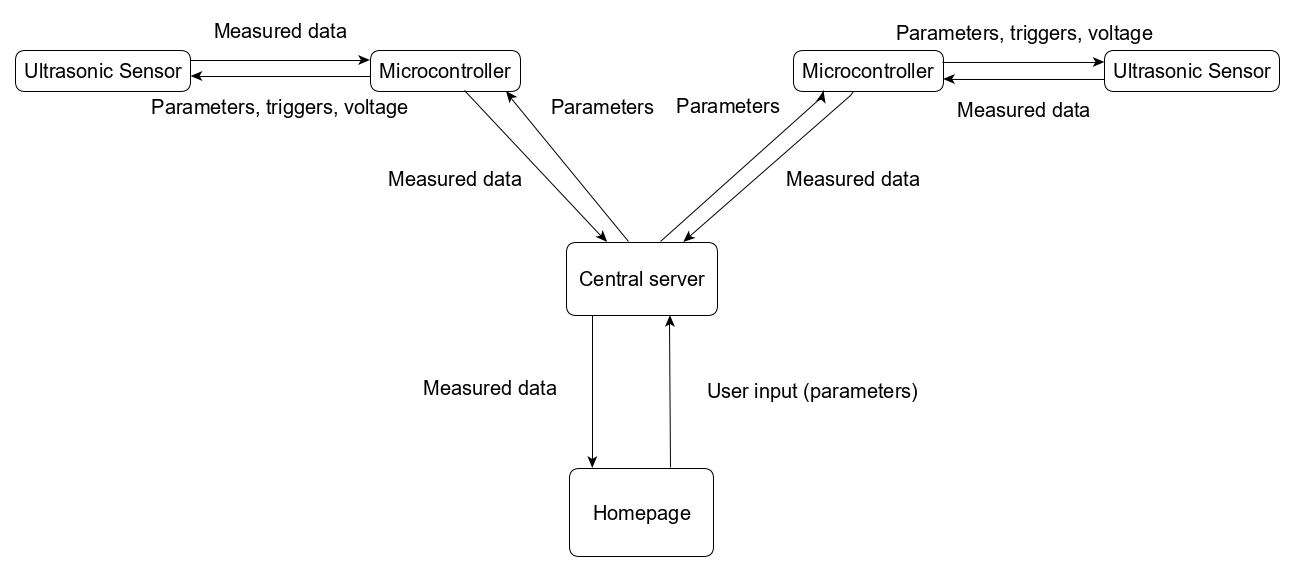
\includegraphics[scale=0.325]{images/circuit3.png}
\caption{Hardware scheme}
\end{figure}

The basic scheme of system hardware is described as follows: the main components
are the micro-controller as central server, the sensors and a web-page. The
sensors must be able to connect to the servers by a WiFi-connection and for this
we assume that the connection is robust and will be available in the given
environment. \par

\subsection{Sensor}
We will use an ultrasonic sensor to measure the level of the liquid. An example of the sensor is Ultrasonic Sensor Module HC-SR-04 by Robokart. 
We want to choose this approach because it is one of the best ways to sense proximity and detect levels with high reliability. Every sensor is connected to a microcontroller 
that collects the data and sends them to the central server via WiFi.  

Every container will have a microcontroller that is connected to at least one sensor (see figure \ref{sensorWithArduino}).
Certain specified heights of minimal and maximal volumes will be set, depending
on various factors, like the position of the container, the probability of it being used, 
the liquid type and as such.

\begin{figure}[h]
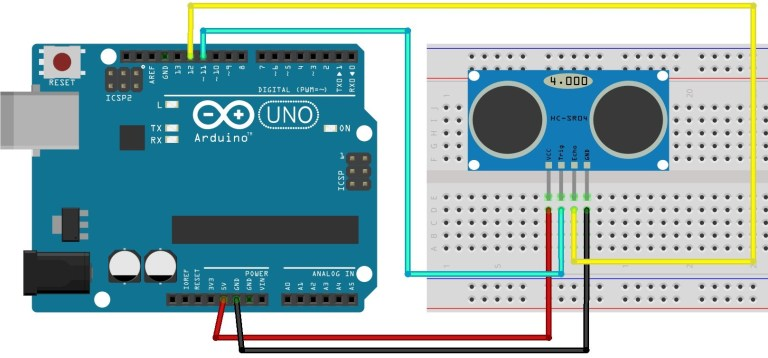
\includegraphics[scale=0.5]{sensorAndArduino.jpg}
\caption{Example of a sensor connected to a microcontroller}
\label{sensorWithArduino}
\end{figure}

\subsection{Central server}

We assume a LAN network to which the controllers and central
server are connected. Through this the microcontrollers will be able to communicate with the
central server by sending continuously the measurements of the liquid heights. 
The central server will perform checks on the thresholds and if needed send an alert to the user. 

As seen in Figure 1, the central server can also host a web page (e.g. with the Node-RED framework) in which the data are visualized in diagrams. 
This will be in an user-friendly interface, for it to be usable by non-technical people also.

\section{Steps of the project}

The first steps of the project will be to research about similar projects and
identifying platforms, programming languages and frameworks, choosing
the most suitable ones for our case.
Furthermore, the connection between devices
plays a crucial role, so we need to know what kind of protocols are needed.

Possible extensions are to also give specific numbers of the height of the
containers, how much volume they contain.
It is also possible to set up LEDs; their light will warn about specific
situations, e.g. when a container is empty a green light is shown, a red one when
is full.

\textcolor{red}{\textbf{\hl{Complete list of components that will be used, with a short description and why}}}

List of ordered components
\begin{itemize}
\item NodeMCU DevKit v1.0 development board (ESP8266) - we will use the microcontroller connected to sensor. It collects and sends data to broker
%Arduino UNO development board - 
\item Infrared proximity sensor (digital / analog output module) - the main sensor to measure the height of the object
\item Rechargeable battery - power source for the microcontroller and sensor
\item Battery charge controller - for the battery
\item Small materials: 
	\begin{itemize}
		\item cables - to connect sensor and microcontroller
		\item breadboard - to connect sensor and microcontroller
		\item LEDs - to signal certain thresholds
		%push button - a button is always useful
	\end{itemize}
\end{itemize}

\textcolor{red}{\textbf{\hl{Complete wiring scheme }}} - will be documented during the implementation 
\begin{itemize}
	 \item Flowchart of operation  
	\begin{figure}[h]
		\center
		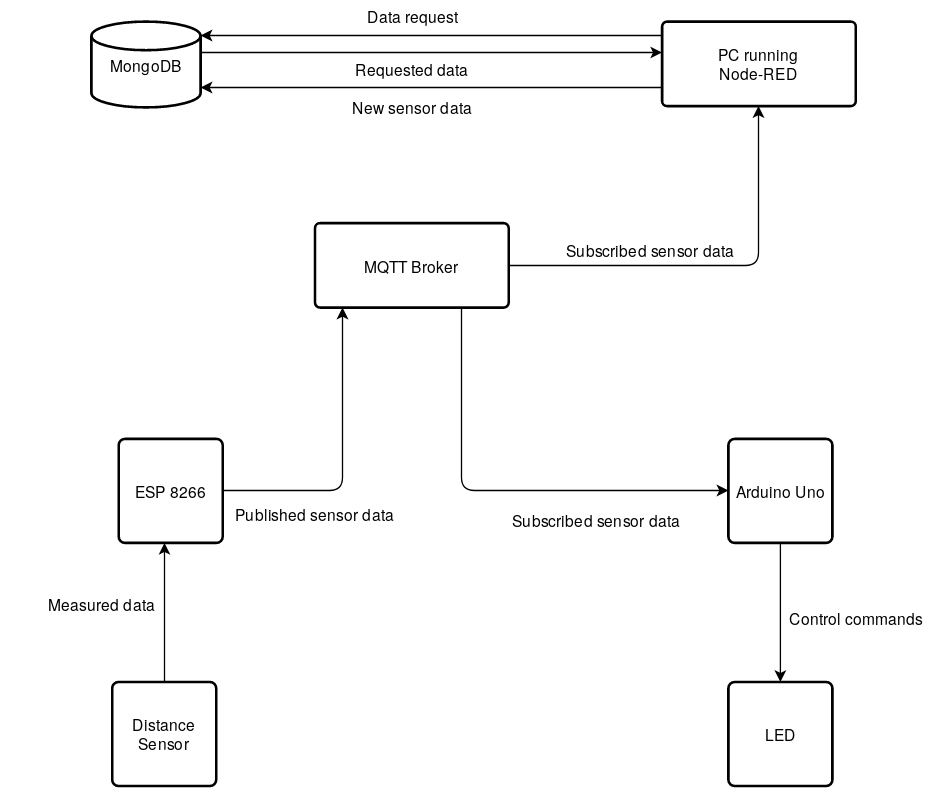
\includegraphics[scale=1]{flow.png}
		\caption{first draft of the flow chart}
		\label{sensorWithArduino}
	\end{figure}
	\item Another entry in the list
	\item List of functions used to communicate with the sensors, including input / output parameters and operation.
	\item List of functions that will be used to communicate with the base station, including input / output parameters and operation. 
	\item Other functions necessary for device operation
	\item Other technical considerations of the devices not described above. 
\end{itemize}
	
\textcolor{red}{\textbf{\hl{Base station documentation:}}} - will be documented during the implementation
\begin{itemize}
	\item Scheme of the software components that run on the base station and how they are related to each other (Broker MQTT, Node-RED, Mongodb?). 
	\item List of functions (flows) themselves to be used to communicate with devices, including input parameters / output (messages) and operation.
	\item List of functions (flows) themselves to be used to communicate with the database and the SCADA, including parameters input / output (messages) and operation. 
	\item Other own functions necessary for the operation of the base station
	\item Other technical considerations not described above. 
\end{itemize}
\textcolor{red}{\textbf{\hl{Device-base station interface. (Message structure)}}}

\textcolor{red}{\textbf{\hl{User manual:}}}
\begin{itemize}
	\item System installation, specifications and calibration
	\item System use and maintenance manual
	\item Detection and solution of possible errors
\end{itemize}

\subsection{Node-RED}
x

\subsection{Arduino}
x

\section{Experiments and Results}

\section{Summary}

\begin{comment}
Project : Height / capacity monitor
Using an ultrasonic sensor or similar, monitor the height of a water tank, paper stack, garbage container, or similar. Think of multiple sensors to map the height in different positions of the container or different containers. To properly manage the filling / emptying of the container, monitoring the tank capacity, etc. Local warning by LEDs, minimum / maximum level alarms, etc.

How is the document going to be valued?

Well written and clear
	Good: The document has no misspellings, and a simple language is used that is perfectly understood. The document is careful: it looks nice, the sheets, drawings, etc., are numbered, the different sections are clearly marked. It shows that they have taken it seriously.
	Enough: The document is understood quite well, although there is some part that can be improved. I found some error, probably attributable to a mistake. With a little more effort, it could have been better.
	Insufficient: I have found several spelling mistakes, and I have not understood many of the things that are said in the document. The document is quite neglected. It shows that they have not tried very hard.


Adequate content
	Good: The document includes complete information on all the points that were requested. They also explain and briefly justify the decisions made.
	Enough: The document includes all the points, but the information is not complete in no more than three of them, or some point is missing. I see some dark aspects in the description of some point. Some key decisions are not justified
	Insufficient: More than one point is missing or the description is quite incomplete 


Good and effective approach
	Good: The approach is good. I can't think of many improvements. The scheme and operation is clear and reasonable. The functions that will be used are well described, with a clear comment on what they do. With this information I think that I would have no difficulty in making the design myself.
	Enough: I think the proposal is good although it admits some improvements. I understand well what they want to do, but if I had to implement it, I would have to ask for some additional clarification.
	Insufficient: The approach is not good. I do not understand the purpose or need of some of the elements of the structures, or of some of the procedures and functions. If I had to implement the application, with this information I would not know where to start.

\end{comment}

\begin{comment}
\maketitle
\newpage

\pagenumbering{arabic} %show page numbers in arabic
\tableofcontents % from the section headings
\newpage

\listoffigures
 
\listoftables

%\listoftables
\newpage

\subfile{einleitung/einleitung}
\newpage

\subfile{grundlagen/grundlagen}
\newpage

\subfile{analyse/analyse}
\newpage

\printbibliography

\subfile{entwicklung/entwicklung}
\newpage

\subfile{evaluation/evaluation}
\newpage

\subfile{zusammenfassungundausblick/zusammenfassungundausblick}
\newpage

\end{comment}

\end{document}